%% USPSC-Introducao.tex

% ----------------------------------------------------------
% Introdução (exemplo de capítulo sem numeração, mas presente no Sumário)
% ----------------------------------------------------------

\chapter[Introdução]{Introdução} \label{cap:introducao}

    A tecnologia atual tem impulsionado significativamente o nível da troca de informações nas mais diversas áreas do mundo, provocando mudanças substanciais em nossa forma de viver, enfrentar desafios e nos relacionar. Especialmente no setor industrial, essa transformação exige uma gestão de dados que esteja intrinsecamente vinculada ao aprimoramento da eficiência e produtividade.
    
    Esse movimento de transformação digital ficou conhecido como a quarta revolução industrial, ou \index{Indústria 4.0}Indústria 4.0, caracterizando-se pela integração de tecnologias avançadas, como a internet das coisas industrial (\index{IIoT}IIoT, do inglês \textit{Industrial Internet of Things}), \index{Inteligência Artificial}Inteligência Artificial (AI, do inglês \textit{Artificial Intelligence}) e processamento de dados em larga escala (também denominados como \textit{Big Data} e \textit{Data Warehousing}).
    
    À medida que o número de dispositivos interconectados e a quantidade de dados gerados por esses aumentam exponencialmente, a necessidade de estratégias robustas de \index{Segurança Cibernética}segurança cibernética torna-se igualmente cruciais, a fim de garantir a proteção da ampla exposição dessas informações contra atividades maliciosas e \index{Ataque Cibernético}ataques cibernéticos. De acordo com \citeonline{wef2022}:
    
    \begin{citacao}
        Conforme a sociedade continua a migrar para o mundo digital, a ameaça do crime cibernético se torna grande, custando rotineiramente às organizações dezenas -- até mesmo centenas -- de milhões de dólares. Os custos não são apenas financeiros: infraestrutura crítica, coesão social e bem-estar mental também estão em risco.
    \end{citacao}

    As redes de comunicação industrial não estão imunes aos desafios que surgem com o aumento exponencial na troca de informações. A interconexão de sistemas em um ambiente industrial requer uma abordagem especializada para enfrentar as crescentes \index{Ameaça Cibernética}ameaças cibernéticas que acompanham essa revolução tecnológica. Portanto, é imperativo que as empresas que operam nesse setor invistam e se desenvolvam em duas áreas de tecnologia fundamentais: da informação (\index{Tecnologia da Informação}TI) -- que desempenha um papel crucial na gestão abrangente da informação -- e operacional (\index{Tecnologia Operacional}TO) -- que abrange os Sistemas de Automação e Controle Industrial (\index{IACS}IACS, do inglês \textit{Industrial Automation and Control Systems}) --, a fim de fortalecer os sistemas de defesas existentes ou desenvolver novas metodologias de defesa.
    
    Até muito recentemente, essas duas áreas de tecnologia (\index{Tecnologia da Informação}TI e \index{Tecnologia Operacional}TO) eram separadas nos níveis técnico e organizacional. A transformação digital supracitada gerou alguns gatilhos, principalmente no setor industrial, obrigando as organizações a reverem esse paradigma e liderar projetos de convergência entre os dois mundos \cite{yassine2021}. A \index{Convergência TI/TO}convergência TI/TO, conforme definida na literatura \cite{yassine2021,tian2019,garimella2018}, apresenta um desafio significativo para as empresas ao propor a descompartimentação dos dados e a intercambialidade de pilares (\textit{e.g.}, a implementação da computação em nuvem no monitoramento dos processos de \index{IACS}IACS).

    À medida que os processos oriundos dessa convergência se tornam mais precisos e complexos, aumenta-se a relevância da transmissão de dados entre os equipamentos que os controlam. Assim, os protocolos de comunicação emergem como componentes de importância primordial na \index{Convergência TI/TO}convergência TI/TO, pois desempenham um papel fundamental na viabilização da integração eficiente e segura entre esses dois domínios. A interoperabilidade e a intercambialidade de um sistema, antes não apresentadas por protocolos industriais proprietários passam a ser características fundamentais nesse contexto. Desse modo, o protocolo \index{OPC UA}OPC UA (do inglês \textit{Open Platform Communications Unified Architecture}) assume uma posição de destaque e relevância ao estabelecer as bases para a troca contínua, segura e confiável de informações entre dispositivos e sistemas de diferentes origens e finalidades.

    O \index{OPC UA}OPC UA é um protocolo de comunicação amplamente utilizado para aplicações \index{IIoT}IIoT e de automação industrial, no qual foi projetado para fornecer uma camada de comunicação segura e confiável para os cenários da \index{Indústria 4.0}Indústria 4.0. Sua construção baseou-se nas seguintes preocupações de segurança, de acordo com \citeonline{pocock2014}: autenticação de usuários/instâncias de aplicativos (software), confidencialidade e integridade ao assinar e criptografar mensagens, disponibilidade por meio de processamento mínimo antes da autenticação e auditabilidade por eventos de auditoria definidos para operações \index{OPC UA}OPC UA. Assim, o OPC UA é amplamente reconhecido como um protocolo seguro, uma vez que incorpora todos os elementos fundamentais para assegurar a comunicação industrial, conforme identificado por \citeonline{lange2010}. Esse conjunto de medidas de segurança o torna um pilar confiável para a infraestrutura de comunicação em ambientes industriais modernos, cuja integridade e segurança dos dados são de suma importância.

    No entanto, a despeito dessa concepção robusta e meticulosamente direcionada para a segurança que caracteriza o protocolo \index{OPC UA}OPC UA, é imperativo reconhecer a dinamicidade do cenário atual de \index{Segurança Cibernética}segurança cibernética. A evolução tecnológica supramencionada e as táticas adversárias à ética podem resultar no surgimento de novas \index{Ameaça Cibernética}ameaças e \index{Vulnerabilidade}vulnerabilidades a esse protocolo, além da possibilidade de ser significativamente afetado por diversas opções de configuração de segurança. Logo, uma postura proativa é crucial para continuar mitigando as \index{Ameaça Cibernética}ameaças emergentes e assegurando a resiliência desse ecossistema industrial. A vigilância e a análise de novas vulnerabilidades são indispensáveis para o aprimoramento contínuo do \index{OPC UA}OPC UA.

    A análise sistemática de \index{Vulnerabilidade}vulnerabilidades proporciona uma visão crítica das possíveis brechas que possam surgir, permitindo uma abordagem preventiva e corretiva na implementação de soluções adequadas. Ao identificar potenciais pontos de risco no protocolo industrial, é possível adotar medidas de segurança proativas, tais como atualizações sistêmicas ou estruturais, ajustes de configuração e o estabelecimento de políticas rigorosas. Essa análise, uma vez bem executada, não apenas identifica fragilidades, mas também orienta as estratégias de proteção, conferindo à organização uma posição privilegiada para agir de maneira ágil e eficaz contra uma \index{Ameaça Cibernética}ameaça ou \index{Ataque Cibernético}ataque cibernético.

    Neste trabalho, uma análise de \index{Vulnerabilidade}vulnerabilidades em redes industriais \index{OPC UA}OPC UA é realizada com o intuito de fornecer uma abordagem estruturada de avaliação da segurança do protocolo. Adota-se a criação de uma bancada experimental como ambiente industrial de simulação de \index{Ataque Cibernético}ataques cibernéticos. Ao aplicar a abordagem proposta, pretende-se contribuir para o fortalecimento da resiliência dessas redes, assim como colaborar com o desenvolvimento do OPC UA.

    % Neste estudo, propomos um framework para análise de vulnerabilidades no protocolo OPC UA e modelagem de ameaças. Também apresentamos cenários de vulnerabilidades identificadas de acordo com a modelagem de ameaças e sugerimos contramedidas através do processo de prova de conceito para cada cenário configurado.
    
    \section{Motivação e Justificativa} \label{sec:motivacao}

    A investigação de trabalhos na comunidade científica foi utilizada como justificativa para a dissertação e motivação para o tópico proposto. Duas buscas principais foram realizadas para que o tema do trabalho fosse definido: a primeira (I) relacionada ao panorama, desafios e oportunidades do protocolo \index{OPC UA}OPC UA no cenário atual, e a segunda (II) com foco no principal gargalo do protocolo observado na pesquisa anterior.
    
    Mediante uma pesquisa sistemática de publicações relacionadas ao protocolo OPC UA na base de dados IEEE Xplore, considerando publicações entre os anos de 2018 e 2022, escritas em inglês e aplicando critérios de exclusão, 238 publicações (artigos, jornais, revistas, atas de conferências, etc.) foram classificadas em categorias, e seus resultados apresentados e discutidos a fim de fornecer uma visão geral do protocolo e investigar os desafios e oportunidades de sua aplicação em ambientes industriais atuais.

    Inicialmente, utilizaram-se diferentes formas de escrita para o termo \index{OPC UA}`OPC UA', como `OPC-UA', `OPC:UA' e `OPC \textit{Unified Architecture}', resultando em 263 publicações. A relevância das publicações foi avaliada e, posteriormente, os seguintes critérios de exclusão foram aplicados para eliminar aquelas que não forneciam informações pertinentes:

    \begin{itemize}
        \item O foco principal da publicação não é em redes de comunicação industrial ou em Internet das Coisas (\index{IoT}IoT, do inglês \textit{Internet of Things}), apesar de o \index{OPC UA}OPC UA ser utilizado no projeto de pesquisa;
        \item O \index{OPC UA}OPC UA é referenciado na publicação, mas não é um tópico relevante dela;
        \item Publicações que se concentram em \textit{marketing} de produtos e não priorizam o \index{OPC UA}OPC UA como protocolo central ou recurso.
    \end{itemize}

    Após a aplicação dos critérios supracitados, um total de 238 publicações foi identificado e submetido a uma análise quantitativa. Entre as publicações selecionadas, 227 (95\%) foram publicadas em anais de conferências, enquanto 11 (5\%) foram publicadas em revistas científicas. A distribuição das publicações por jornais e conferências por ano é ilustrada na \autoref{fig:pubPorAno}.

    % {\color{red}
    % A principal revista científica que apresenta artigos relacionados ao OPC UA é `\textit{IEEE Access}', com um total de seis publicações. O \textit{IEEE Access} é uma revista arquivística multidisciplinar, de acesso aberto (OA, do inglês \textit{Open Access}), orientada para aplicações, completamente eletrônica, que apresenta continuamente os resultados de pesquisas ou desenvolvimentos originais em todos os campos de interesse do IEEE \cite{access2023}. 
    
    % Em relação a conferências, simpósios e congressos, a principal conferência para pesquisas relacionadas ao OPC UA foi encontrada na `\textit{IEEE International Conference on Emerging Technologies and Factory Automation (ETFA)}', com um total de 57 publicações. Este número é notável, pois representa 25,1\% de todos os artigos de conferência.
    % } % Fim da cor vermelha

    \begin{figure}[htbp]
        \caption{Número de publicações relacionadas ao OPC UA por ano}
        \label{fig:pubPorAno}
        \begin{center}
            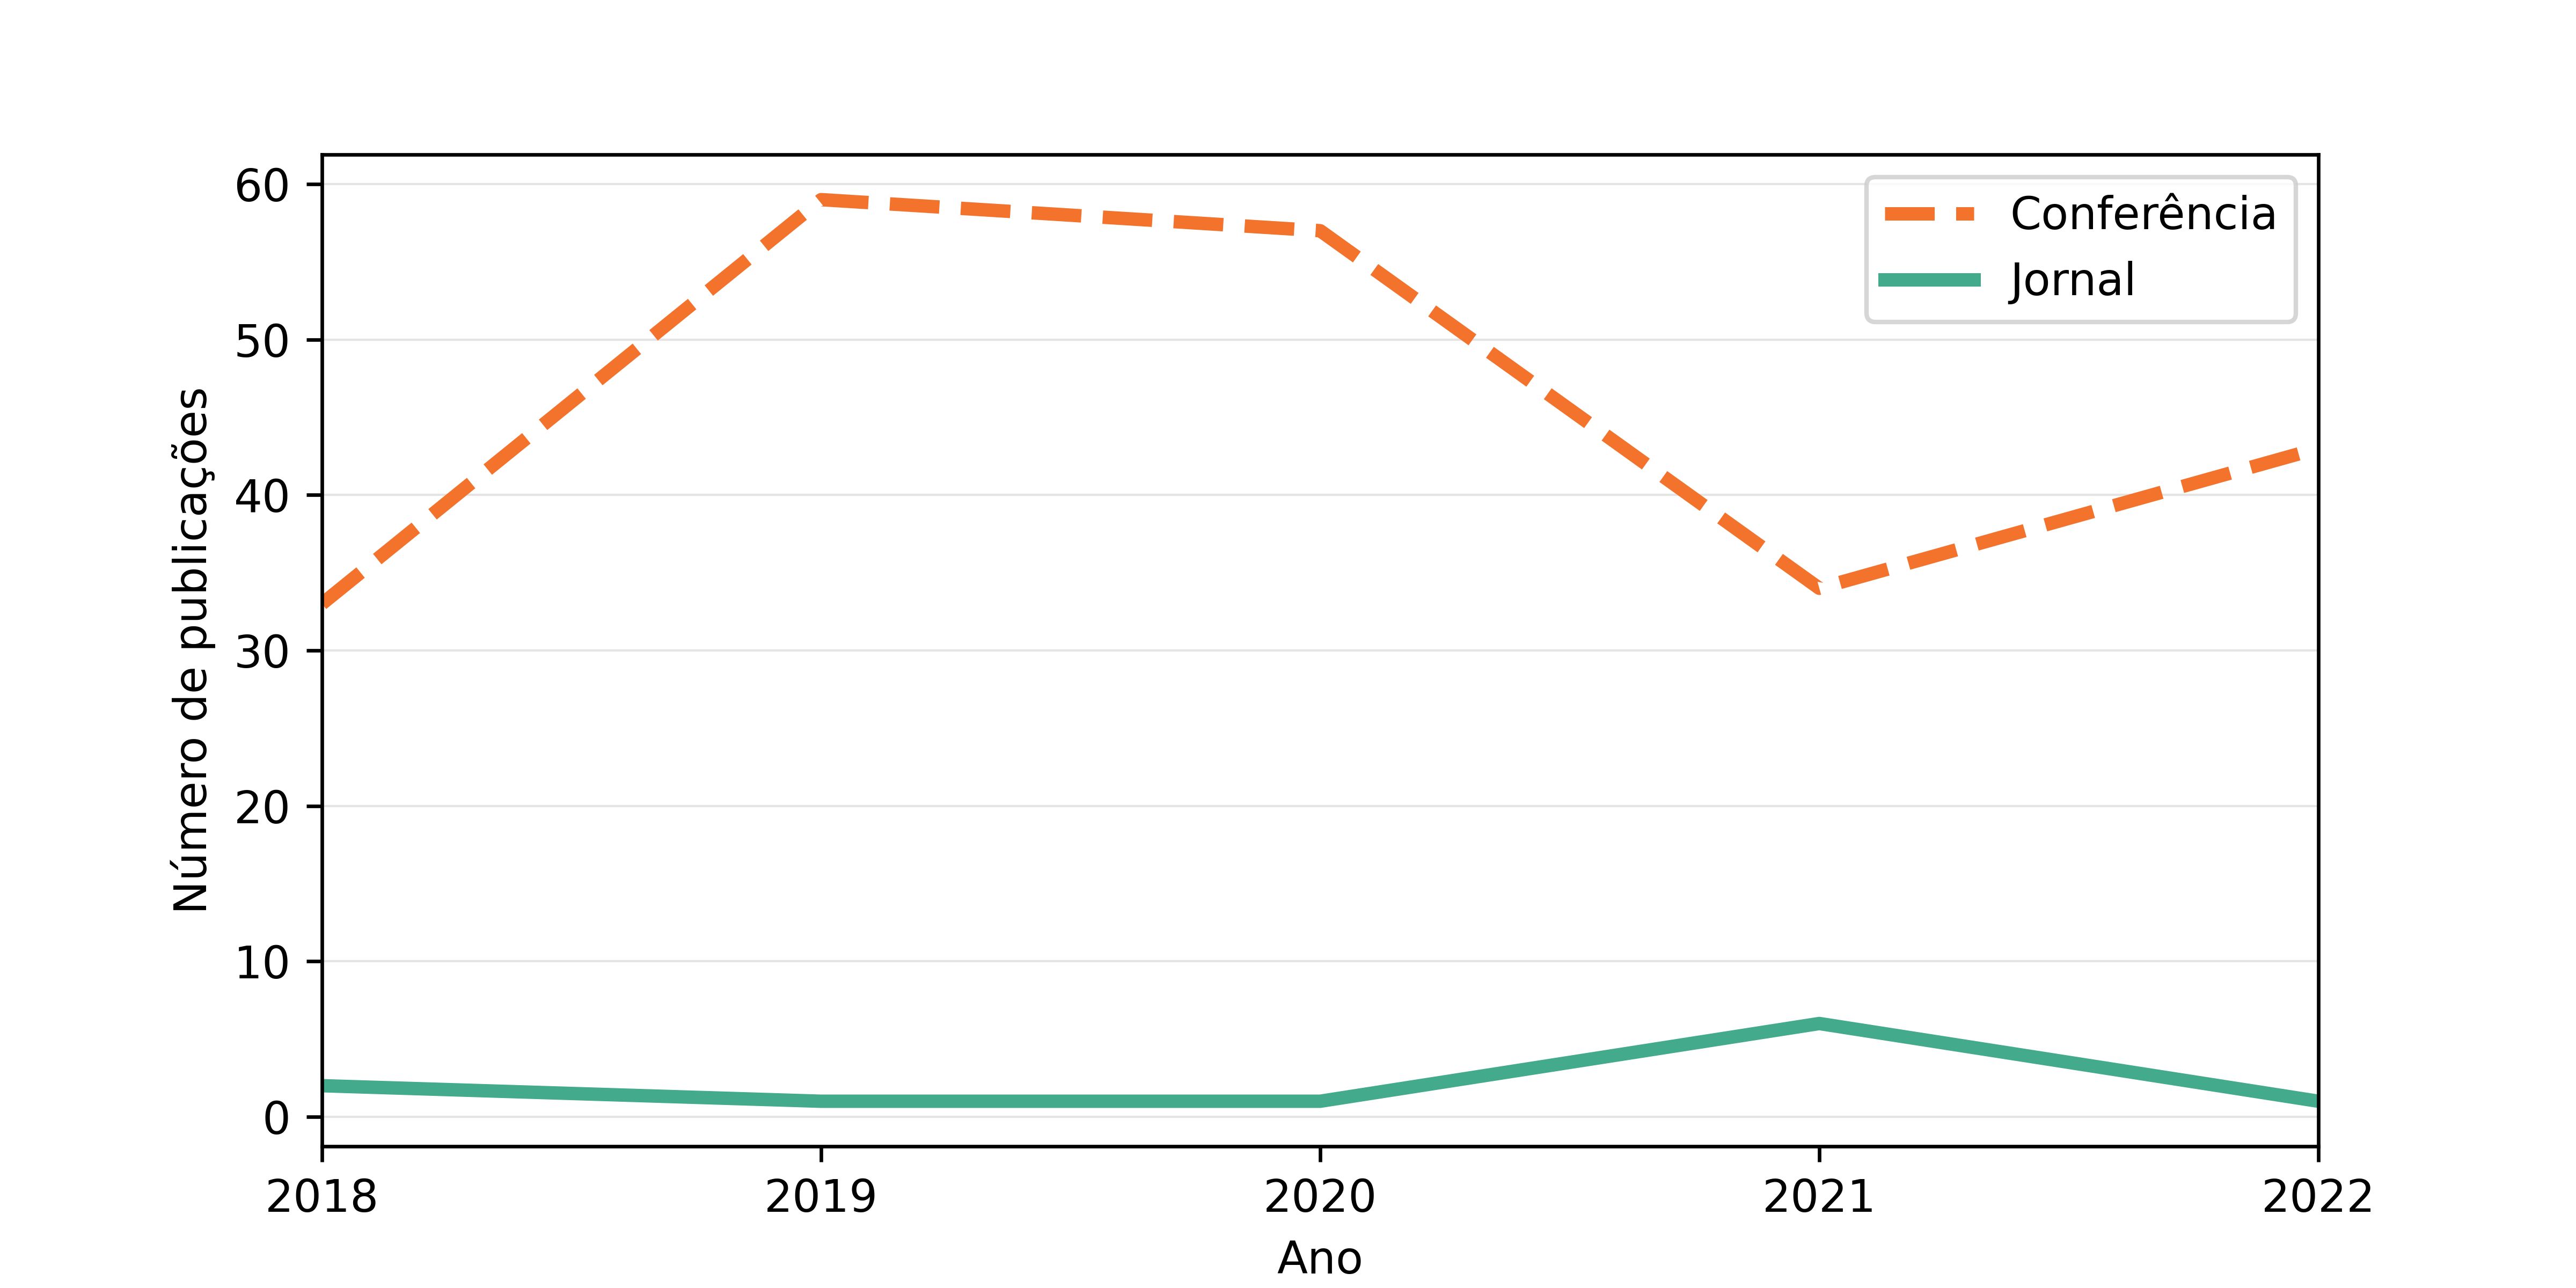
\includegraphics[width=0.7\linewidth]{USPSC-img/pubPerYear.png}
        \end{center}
        \fonte{elaborada pelo autor.}
    \end{figure}

    Após uma leitura e análise cuidadosas, as publicações identificadas foram classificadas nos tópicos sugeridos, conforme apresentado abaixo, seguidos de suas respectivas descrições:

    \begin{itemize}
        \item \underline{Integração e Teoria (TI)}: integração do protocolo com diferentes sistemas, dispositivos e aplicativos por meio de um modelo de dados comum, assim como sua teoria baseada em padrões como IEC 61499 e IEC 62541 e trabalhos de pesquisa existentes;
        \item \underline{Desenvolvimento de Produto (PD)}: criação de novos servidores, clientes, \textit{frameworks} e modelos de informação para expandir a funcionalidade e compatibilidade do \index{OPC UA}OPC UA, fornecendo uma base para novos sistemas e aplicativos industriais;
        \item \underline{Segurança (S)}: enfatiza significativamente a segurança, utilizando autenticação, criptografia e controle de acesso para proteger os dados e sistemas industriais contra \index{Ameaça Cibernética}ameaças cibernéticas, ou analisando as implicações de segurança da implementação do protocolo em um sistema;
        \item \underline{Análise de Desempenho (PA)}: análise do desempenho do protocolo, identificação de gargalos e indicação de possíveis melhorias para o desempenho geral do sistema, utilizando medidas como latência, variação de latência, perda de pacotes, taxa de transferência, entre outras métricas para avaliar o comportamento do sistema e verificar a conformidade com os requisitos aplicáveis;
        \item \underline{Comparação de Protocolo (PC)}: comparação com outros protocolos de comunicação industrial e \index{IoT}IoT, principalmente com base em indicadores de desempenho;
        \item \underline{Diagnóstico e Monitoramento (DM)}: oferece recursos de diagnóstico e monitoramento, tais como monitoramento da saúde do sistema, gerenciamento de alarmes e notificação de eventos, a fim de garantir a disponibilidade do sistema e reduzir o tempo de inatividade;
        \item \underline{Comunicação \textit{Wireless} (W)}: principal característica da rede é a utilização do protocolo \index{OPC UA}OPC UA através de uma comunicação sem fio;
        \item \underline{Outros (O)}: abrange uma ampla gama de áreas de pesquisa relacionadas à tecnologia \index{OPC UA}OPC UA, como modelagem de dados, interoperabilidade semântica, virtualização, computação em nuvem e computação de borda.
    \end{itemize}

    A presente análise possui implicações significativas para a identificação de lacunas no estado atual da pesquisa na comunidade científica. Um artigo intitulado "A Survey on OPC UA Protocol: Overview, Challenges and Opportunities" \cite{daSilva2023} foi desenvolvido e publicado na \textit{IEEE/IAS International Conference on Industry Applications}, apresentando uma discussão mais aprofundada e integrada dos trabalhos atuais em cada categoria. A literatura existente sobre \index{OPC UA}OPC UA é notavelmente carente de trabalhos que explorem a interseção entre segurança e comunicação sem fio, o que representa uma lacuna crítica. A \autoref{tab:paperCategory} fornece um resumo abrangente dos tópicos abordados nas publicações identificadas ao longo do período estudado, permitindo uma avaliação sistemática das tendências e padrões na comunidade científica ao longo dos últimos anos.
    
    \begin{table}[htbp]
        \centering
        \caption{Quantidade de publicações por categorias}%
	\label{tab:paperCategory}
        \begin{tabular}{ccccccccc}
            \toprule
            \thead{Ano} & \thead{TI} & \thead{PD} & \thead{S} & \thead{PA} & \thead{PC} & \thead{DM} & \thead{W} & \thead{O} \\
            \toprule
            2018 & 14 & 12 & 4 & 5  & 2  & 2  & 2 & 6 \\
            \midrule
            2019 & 21 & 20 & 6 & 10 & 10 & 10 & 8 & 10 \\
            \midrule
            2020 & 22 & 13 & 6 & 8  & 10 & 13 & 6 & 15 \\
            \midrule
            2021 & 17 & 16 & 4 & 12 & 6  & 3  & 7 & 3 \\
            \midrule
            2022 & 12 & 18 & 5 & 7  & 7  & 5  & 3 & 10 \\
            \bottomrule
            \textbf{Total} & 86 & 79 & 25 & 42 & 35 & 33 & 26 & 44 \\
            \bottomrule
        \end{tabular}
        \fonte{elaborada pelo autor.}%
    \end{table}

    A segurança tem historicamente recebido uma proporção menor de atenção na área de pesquisa. Isso pode ser atribuído ao fato de que o OPC UA foi projetado para incorporar medidas de segurança, incluindo criptografia, autenticação e autorização \cite{lange2010}. Tal abordagem abrangente de segurança, aliada às recomendações e diretrizes de melhores práticas fornecidas pela fundação desenvolvedora \textit{OPC Foundation}, contribuiu para uma redução notável na quantidade de pesquisas dedicadas especificamente a esse tópico.

    % {\color{red}
    % A pesquisa futura pretende aprofundar nas preocupações com a segurança por meio de uma análise quantitativa semelhante à primeira, especificamente nas produções relacionadas à detecção de intrusão ou anomalias neste tipo de rede.
    
    % É importante notar que algumas publicações foram classificadas em mais de uma categoria, indicando a natureza multidisciplinar da pesquisa em torno da tecnologia OPC UA, bem como a predominância de estudos relacionados à integração ao longo das décadas. Uma das razões para isso é o contínuo surgimento de novas tecnologias que complementam a usabilidade do protocolo, introduzindo novas funcionalidades ao sistema geral.

    % A quantidade de estudos sobre o desenvolvimento de produtos é um tópico significativo, o que é refletido pelo número substancial de pesquisas dedicadas à teoria e integração do protocolo com outras tecnologias. Isso é ainda suportado pela projeção feita por \citeonline{industryarc2023}, que estima que o mercado de rede OPC UA experimentará uma taxa de crescimento anual composta (CAGR) de 6,3\% durante o período de previsão de 2021 a 2026, resultando em um tamanho de mercado esperado de US\$ 18,3 bilhões até 2026.
    
    % Embora a análise de desempenho, comparação entre protocolos, diagnóstico e monitoramento sejam áreas importantes de pesquisa, isso não significa que sejam mais significativas do que outros tópicos menos explorados, como segurança e comunicação sem fio. Ainda que o OPC UA tenha sido projetado com uma forte base em segurança e comunicação sem fio, pesquisas adicionais são necessárias para abordar os desafios apresentados pelas tecnologias emergentes, como as redes 5G e TSN, bem como para aprimorar as medidas de cibersegurança. Assim, uma abordagem holística para a pesquisa em OPC UA deve abranger todas essas áreas para garantir a integração perfeita do OPC UA com as tecnologias em evolução da \index{Indústria 4.0}Indústria 4.0.
    
    % As publicações listadas na categoria "Outros (O)", que constituem um número significativo, indicam que o protocolo foi extensivamente estudado em múltiplos domínios dentro da comunidade acadêmica. A literatura sobre este tema tem se concentrado principalmente na aplicação do protocolo em vários contextos.
    % } % Fim da cor vermelha
    
    % \subsection{Pesquisa II}\label{subsec:pesqII}

    As descobertas deste estudo inicial foram significativas ao fornecer uma visão geral e atual do protocolo \index{OPC UA}OPC UA, destacando a necessidade de manter um interesse vigilante na área de segurança, a fim de garantir a resiliência do protocolo frente às constantes ameaças a esses sistemas. Assim, uma nova análise quantitativa foi realizada visando o aprofundamento nos trabalhos com esse enfoque, especificamente naqueles atinentes à segurança cibernética nesse tipo de rede. Para isso, utilizaram-se as bases de dados IEEE Xplore, Web of Science e Scopus.

    Em uma pesquisa inicial, os termos \index{OPC UA}`OPC UA' e `\textit{Security}' foram empregados como palavras-chave, repetindo os mesmos critérios de inclusão relatados na pesquisa anterior. Entretanto, não se aplicou nenhum critério de exclusão. A \autoref{fig:pubAmount} apresenta os resultados separados por ano, de 2013 até o de 2022.

    \begin{figure}[htbp]
        \caption{Quantidade de publicações sobre a segurança em redes OPC UA nos últimos anos}
        \label{fig:pubAmount}
        \begin{center}
            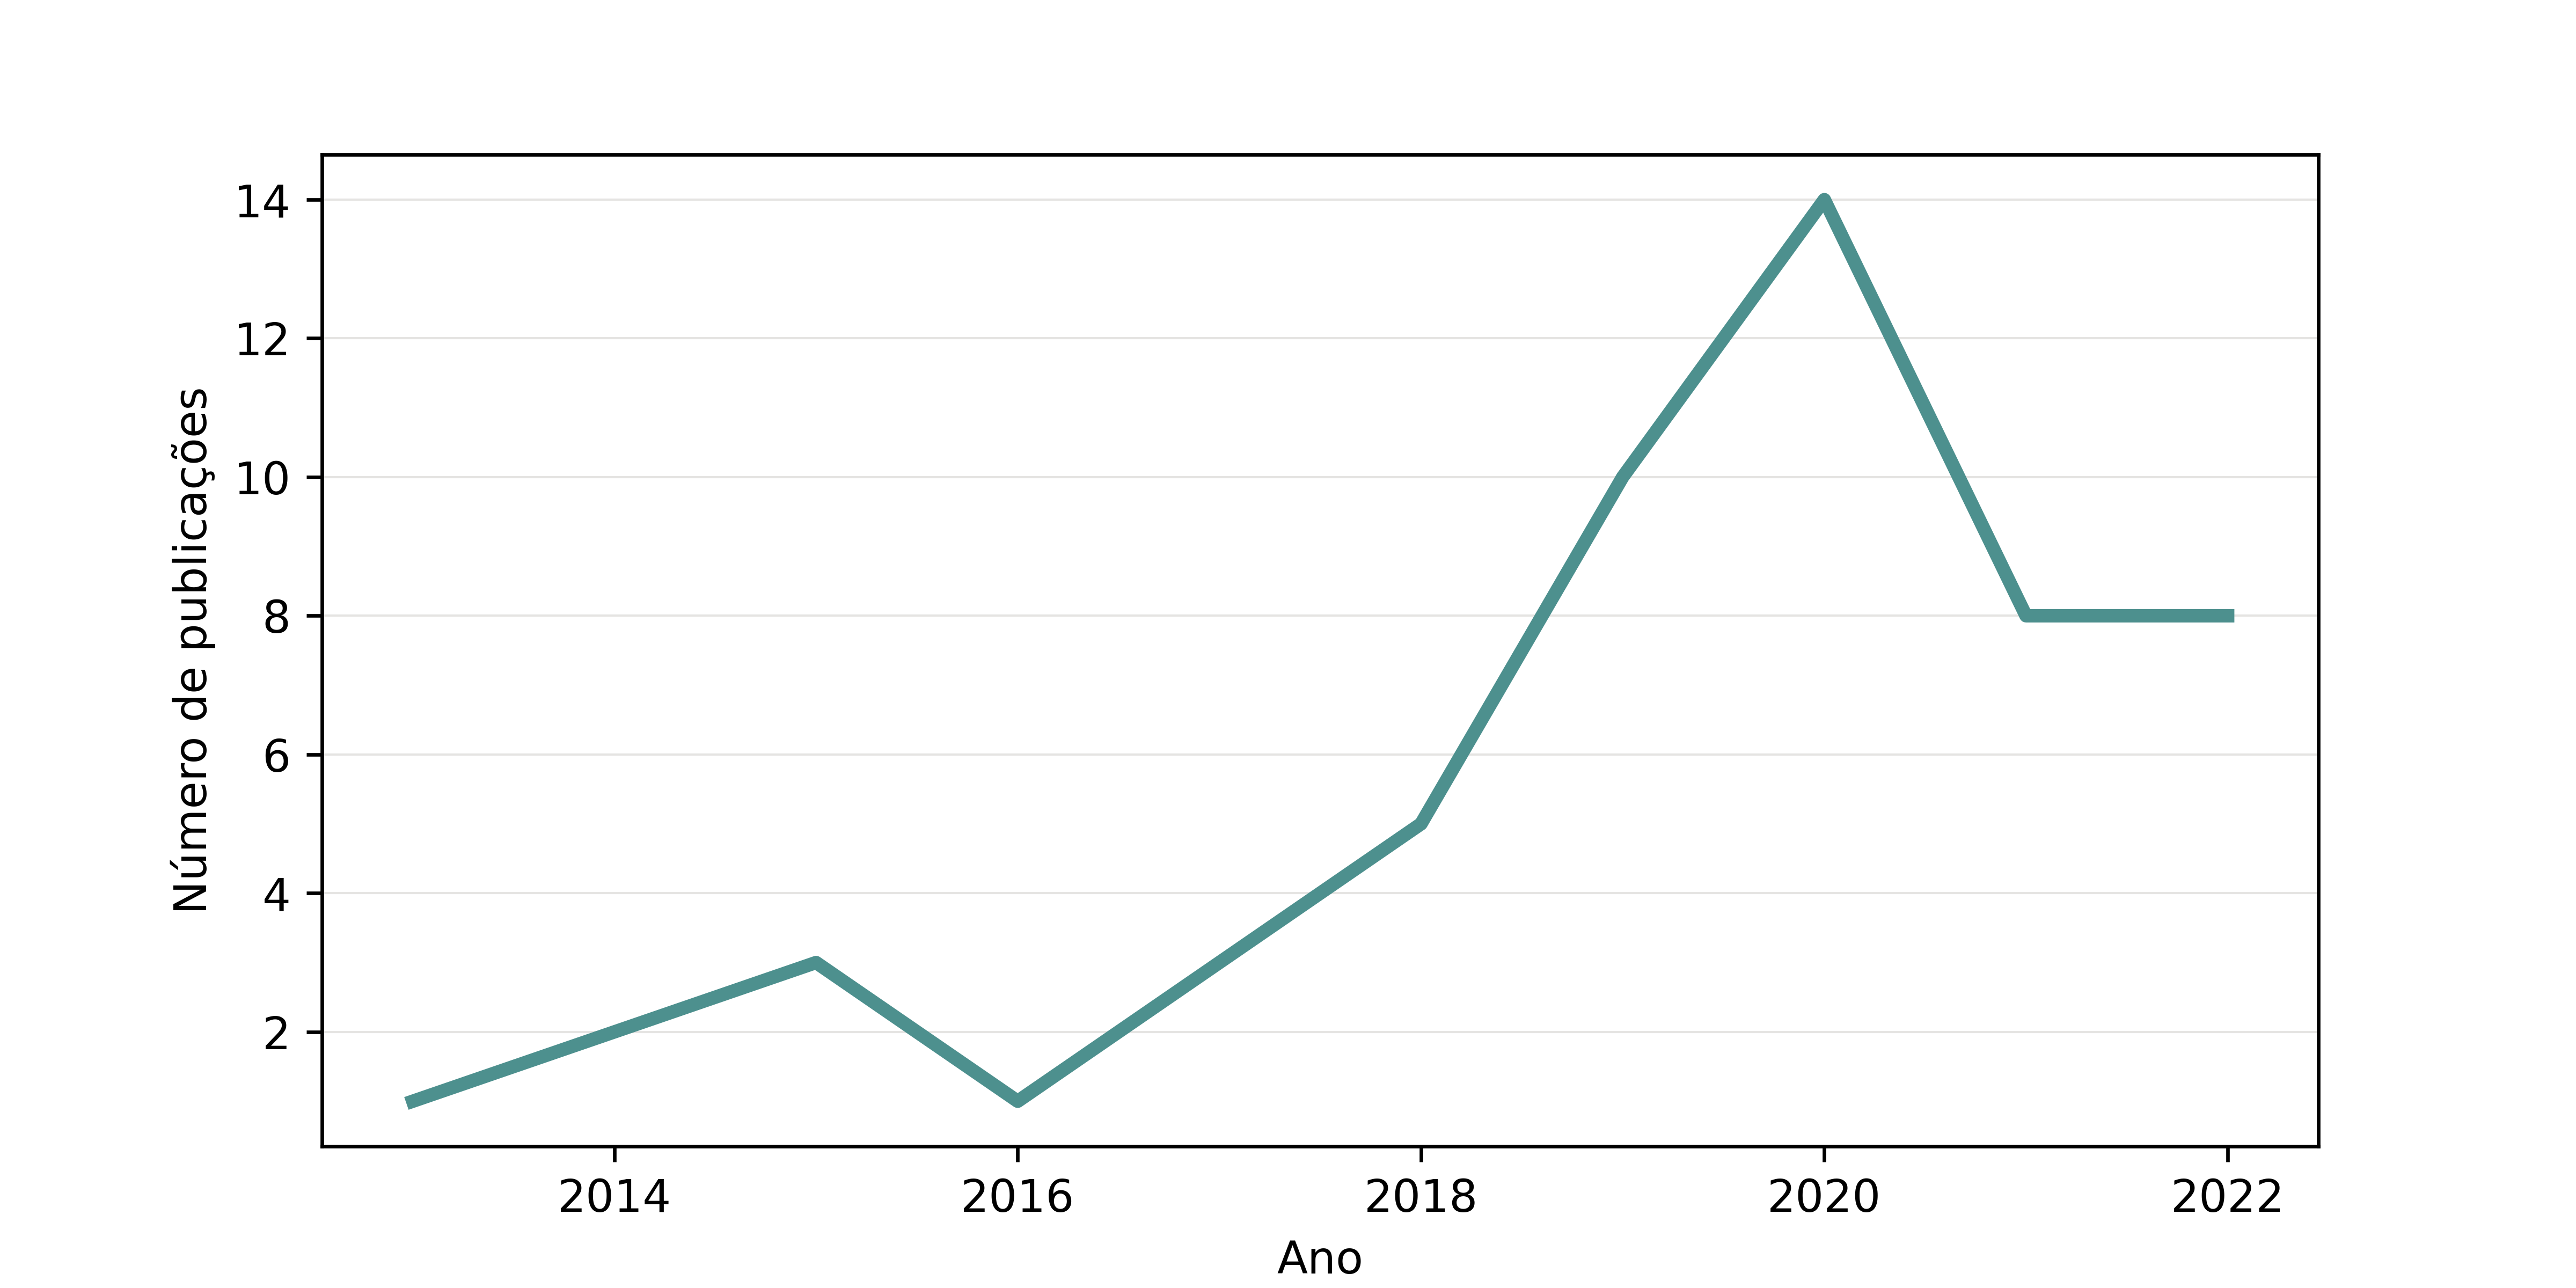
\includegraphics[width=0.7\linewidth]{USPSC-img/pubAmount1.png}
        \end{center}
        \fonte{elaborada pelo autor.}
    \end{figure}

    A análise sobre o panorama das publicações relacionadas à segurança em redes \index{OPC UA}OPC UA ao longo da última década evidencia um notável crescimento na quantidade de trabalhos sobre o tema, indicando um interesse crescente e uma conscientização ampliada acerca dos desafios de segurança envolvendo esse protocolo. No entanto, a partir de 2021, observa-se um fenômeno de diminuição e posterior estagnação nessa produção acadêmica e técnica. Essa tendência decrescente pode derivar de uma combinação de fatores, como a possibilidade de que muitos aspectos cruciais já tenham sido discutidos e explorados, a influência de outros tópicos emergentes na segurança cibernética, ou até mesmo considerações externas que impactaram a dinâmica da pesquisa e das publicações (\textit{e.g.}, pandemia de COVID-19).

    A seguir, a estrutura de pesquisa descrita abaixo foi empregada a fim de filtrar os trabalhos relacionados à análise de \index{Vulnerabilidade}vulnerabilidades em redes \index{OPC UA}OPC UA, aplicando como critérios de inclusão: publicações no período de 2013 a 2022, escritas em inglês. Entende-se `TKA' pela junção dos campos \textit{title}, \textit{keywords} e \textit{abstract}. Os resultados estão descritos na \autoref{fig:pubVulAmount}.

    \begin{minted}[
        breaklines,
        %linenos,
        mathescape,
        encoding=utf8,
        framesep=2mm,
        baselinestretch=1.2,
        bgcolor=codeback,
        fontsize=\footnotesize
    ]{vhdl}
("TKA":“OPC UA” OR "TKA":“OPC-UA” OR "TKA":“OPC:UA” OR "TKA":“OPC Unified Automation”) AND ("TKA":“Vulnerabilities” OR "TKA":“Vulnerabilities Analysis” OR "TKA":“Vulnerabilities Assessment”)
    \end{minted}
    
    \begin{figure}[htbp]
        \caption{Quantidade de publicações sobre vulnerabilidades em redes OPC UA nos últimos anos}
        \label{fig:pubVulAmount}
        \begin{center}
            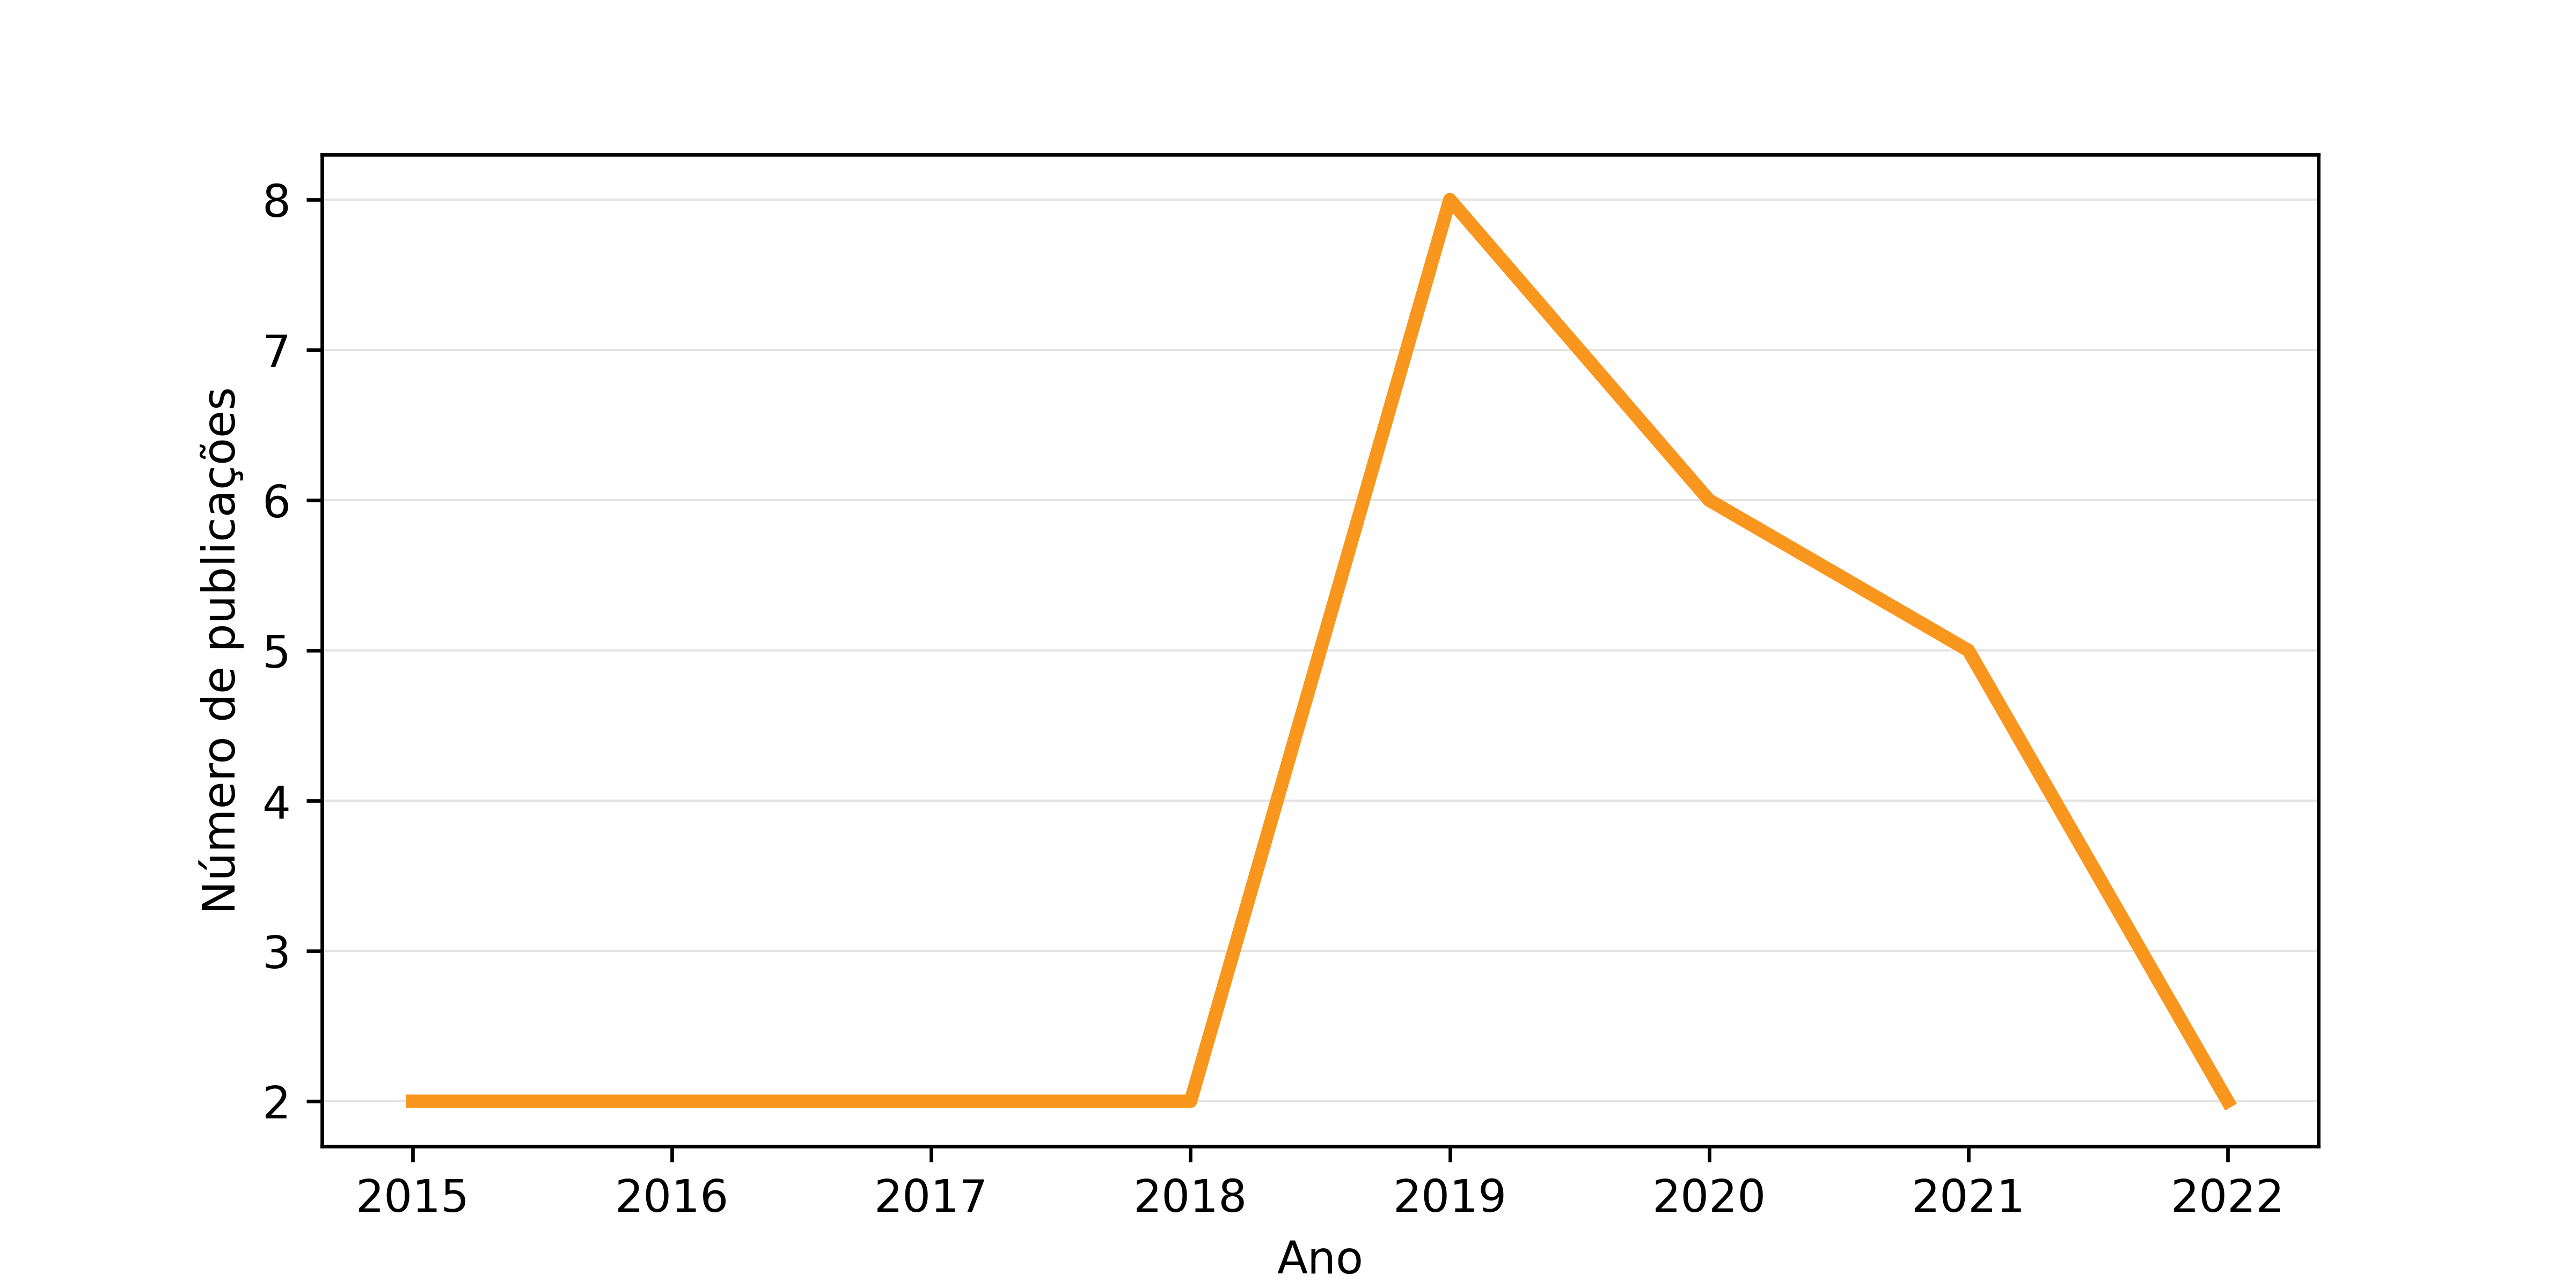
\includegraphics[width=0.7\linewidth]{USPSC-img/pubVulAmount.png}
        \end{center}
        \fonte{elaborada pelo autor.}
    \end{figure}
    
    A avaliação desses resultados conduz a uma conclusão que, embora semelhante à anterior, revela uma oscilação marcante. No ano de 2019, um pico significativo na quantidade de artigos publicados denota um interesse acentuado e um maior reconhecimento por parte da comunidade científica sobre as \index{Vulnerabilidade}vulnerabilidades associadas ao \index{OPC UA}OPC UA. Entretanto, a partir de 2020, constata-se uma inversão na tendência, com uma redução no número de publicações. Esse declínio pode estar relacionado a diversos fatores interconectados, conforme descrito anteriormente. Contudo, vale ressaltar a importância do tema do presente estudo, uma vez que a natureza incerta das ameaças e a dinâmica das vulnerabilidades em ambientes industriais utilizando esse protocolo são bem conhecidas.
    
    \section{Objetivos} \label{sec:objetivos}

    Considerando a relevância do tema, o presente estudo propõe uma investigação detalhada de ataques cibernéticos em redes \index{OPC UA}OPC UA, visando desenvolver, implementar e validar uma bancada experimental para simulações de intrusões em sistemas de automação e controle industriais. Busca-se compreender as potenciais fragilidades que podem comprometer a segurança dessas redes, identificando os principais pontos de risco e explorando possíveis contramedidas para mitigar as \index{Ameaça Cibernética}ameaças detectadas.

    Observa-se um caráter desafiador no objetivo, uma vez que a complexidade e a diversidade dos dados trafegados nas camadas do protocolo demandam um alto grau de especialização em \index{Segurança Cibernética}segurança cibernética e técnicas avançadas de engenharia de redes.

    Dentro desse contexto, os objetivos específicos a serem atingidos pela metodologia proposta são:
    
    \begin{itemize}
        \item Investigar e compreender os princípios e conceitos fundamentais das redes \index{OPC UA}OPC UA, a fim de identificar os principais desafios e \index{Ameaça Cibernética}ameaças relacionados à segurança nestas redes;
        \item Propor e desenvolver uma bancada experimental como ambiente industrial de simulação de \index{Ataque Cibernético}ataques cibernéticos;
        \item Investigar, selecionar e aplicar alguns ataques comuns para IIoT e demonstrar a reação do protocolo OPC UA às intrusões na rede;
        \item Analisar o cenário de ataque do ponto de vista do invasor, a fim de identificar os desafios da segurança, encontrar possíveis novas vulnerabilidades e propor contramedidas para mitigação.
    \end{itemize}
    
    \section{Estrutura dos Capítulos} \label{sec:estCapitulos}

    Esta dissertação está estruturada em capítulos que abordam os diferentes aspectos dos trabalhos desenvolvidos. O \autoref{cap:refTeorico} apresenta uma revisão abrangente da literatura relacionada ao tema, incluindo os conceitos teóricos fundamentais das redes OPC UA, os princípios essenciais da segurança cibernética e as técnicas de análise de vulnerabilidades aplicadas a essas redes. Além disso, são discutidos trabalhos anteriores relevantes para o contexto deste estudo. No \autoref{cap:desenvolvimento}, os principais componentes e materiais empregados na montagem da bancada experimental para a realização dos ensaios de intrusão são detalhados. Ademais, são descritos em pormenor os ataques cibernéticos selecionados e a metodologia adotada para sua análise. Os resultados e discussões são apresentados no \autoref{cap:resultados}, que inclui a implementação da bancada experimental, a aquisição de dados nos cenários de ataques cibernéticos, o processamento dos dados, e a análise dos resultados. Por fim, são propostas melhorias e mitigações, incluindo recomendações para comunicações seguras com o protocolo OPC UA, melhorias na infraestrutura e gestão de redes, e normas e regulamentos. Por fim, o \autoref{cap:conclusao} delineia as considerações finais, incluindo conclusões e sugestões para trabalhos futuros.